\documentclass[tikz, border=10pt]{standalone}
\usepackage{pgfplots}
\pgfplotsset{compat=1.18}
\begin{document}
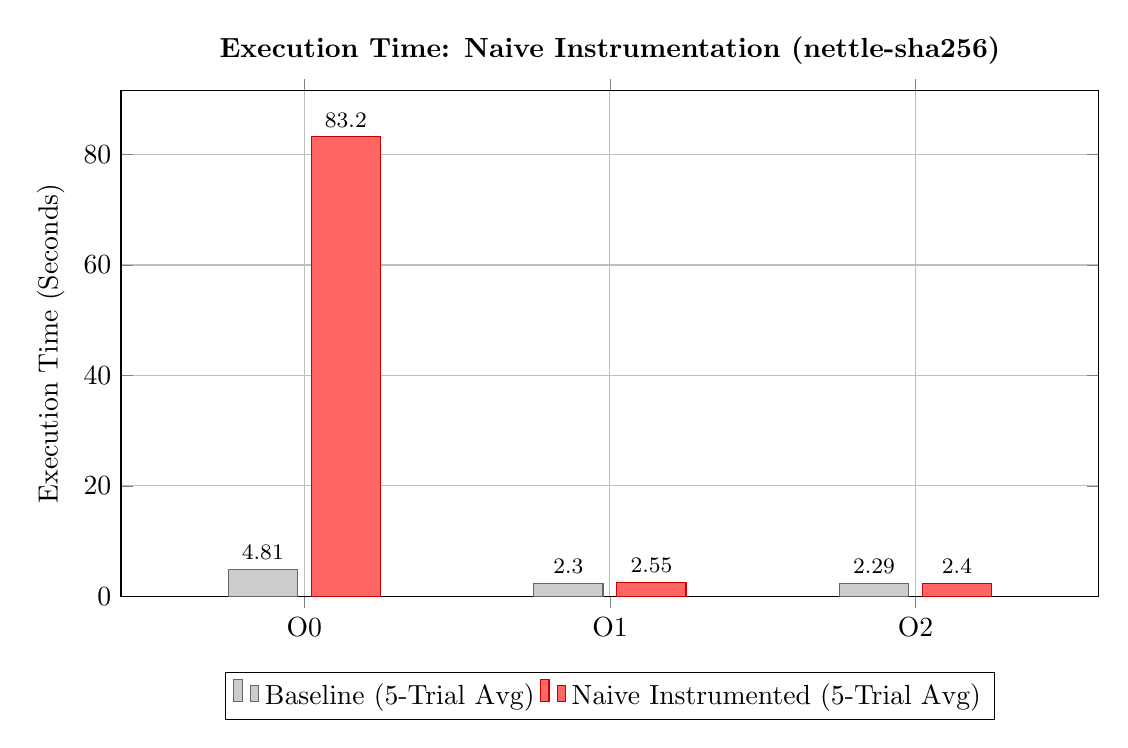
\begin{tikzpicture}
\begin{axis}[
    title={\textbf{Execution Time: Naive Instrumentation (nettle-sha256)}},
    ybar=5pt, enlarge x limits=0.3, ylabel={Execution Time (Seconds)},
    symbolic x coords={O0, O1, O2}, xtick=data, bar width=25pt,
    nodes near coords, every node near coord/.append style={font=\footnotesize},
    legend style={at={(0.5,-0.15)}, anchor=north, legend columns=-1},
    width=14cm, height=8cm, grid=major, ymin=0
]
\addplot[fill=gray!40, draw=gray!80!black] coordinates {(O0, 4.81) (O1, 2.30) (O2, 2.29)};
\addplot[fill=red!60, draw=red!80!black] coordinates {(O0, 83.20) (O1, 2.55) (O2, 2.40)};
\legend{Baseline (5-Trial Avg), Naive Instrumented (5-Trial Avg)}
\end{axis}
\end{tikzpicture}
\end{document}
